\documentclass[titlepage]{scrartcl}
\usepackage{enumitem}
\usepackage[british]{babel}
\usepackage[style=apa, backend=biber]{biblatex}
\DeclareLanguageMapping{british}{british-apa}
\usepackage{url}
\usepackage{float}
\usepackage[labelformat=empty]{caption}
\restylefloat{table}
\usepackage{perpage}
\MakePerPage{footnote}
\usepackage{abstract}
\usepackage{graphicx}
% Create hyperlinks in bibliography
\usepackage{hyperref}
\usepackage{amsmath}

\usepackage[T1]{fontenc}
\usepackage[utf8]{inputenc}
\usepackage{blindtext}
\setkomafont{disposition}{\normalfont\bfseries}

\graphicspath{
    {./resources/},
}
\addbibresource{~/Documents/library.bib}

\newsavebox{\abstractbox}
\renewenvironment{abstract}
  {\begin{lrbox}{0}\begin{minipage}{\textwidth}
   \begin{center}\normalfont\sectfont\abstractname\end{center}\quotation}
  {\endquotation\end{minipage}\end{lrbox}%
   \global\setbox\abstractbox=\box0 }

\usepackage{etoolbox}
\makeatletter
\expandafter\patchcmd\csname\string\maketitle\endcsname
  {\vskip\z@\@plus3fill}
  {\vskip\z@\@plus2fill\box\abstractbox\vskip\z@\@plus1fill}
  {}{}
\makeatother

\DeclareCiteCommand{\citeyearpar}
    {}
    {\mkbibparens{\bibhyperref{\printdate}}}
    {\multicitedelim}
    {}

\begin{document}
    \title{ECS742\\Interactive Digital Media Techniques\\Mini-Assignment 1: Arduino}
    \subtitle{\LARGE{Technical Report}}
    \author{Sam Perry\\160842984}
    \date{}
    \maketitle

    \section{Connecting and reading the FSR}
    Initially, a circuit was created to demonstrate the reading of values from
    the FSR (Force Sensitive Resistor).  A 5V supply was used to pass a current
    through the resistor, which was measured via analog input 0.  A 10kohm
    pulldown resistor was conntected to ground between the FSR and the input.
    This was necessary to avoid a direct connection between the 5V supply and
    ground at points when the FSR provides little to no resistance. This also
    creates a consistantly low value to input when resistance from the FSR
    is high, avoiding unpredicatbale floating readings caused by a disconected
    input.\\
    \begin{figure}[H]
        \makebox[\textwidth]{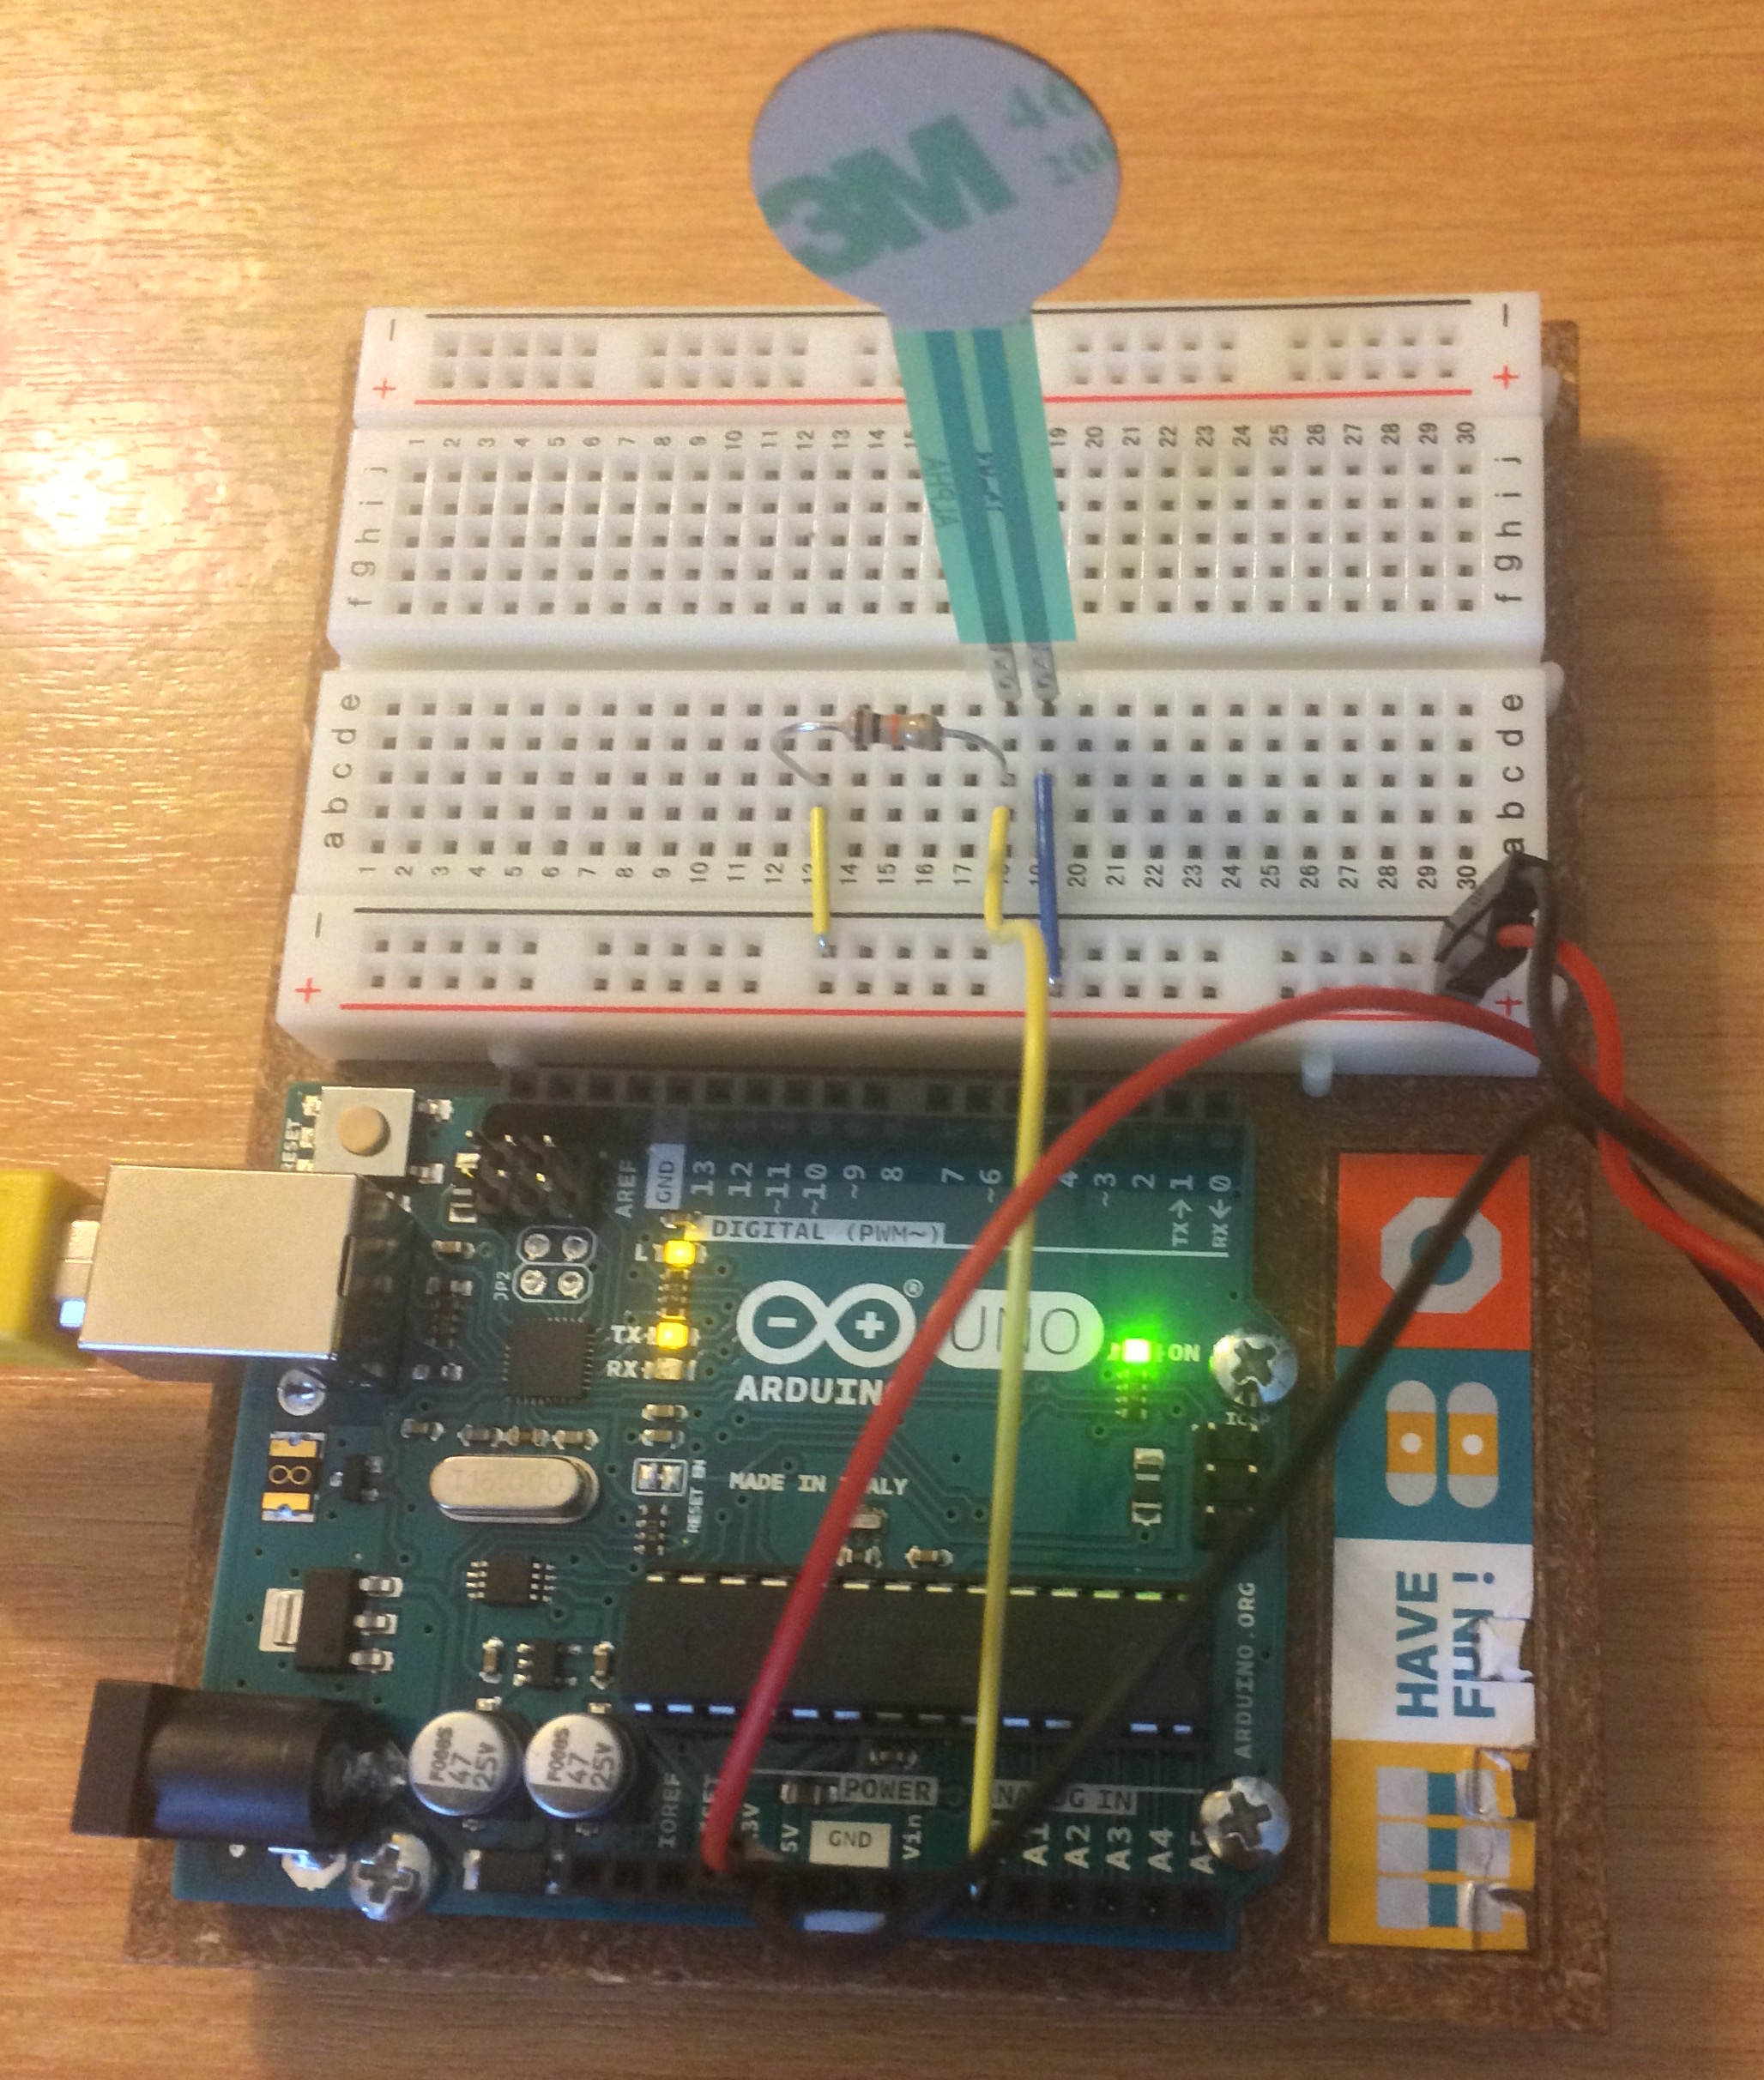
\includegraphics[width=0.35\textwidth]{Step1}}
    \end{figure}

    Code was written to print values to the serial port. A Python script was
    used to record these values as shown:
    \begin{figure}[H]
        \caption{Value measured over time. A sharp increase in preassure followed by a gradual release is displayed.}
        \makebox[\textwidth]{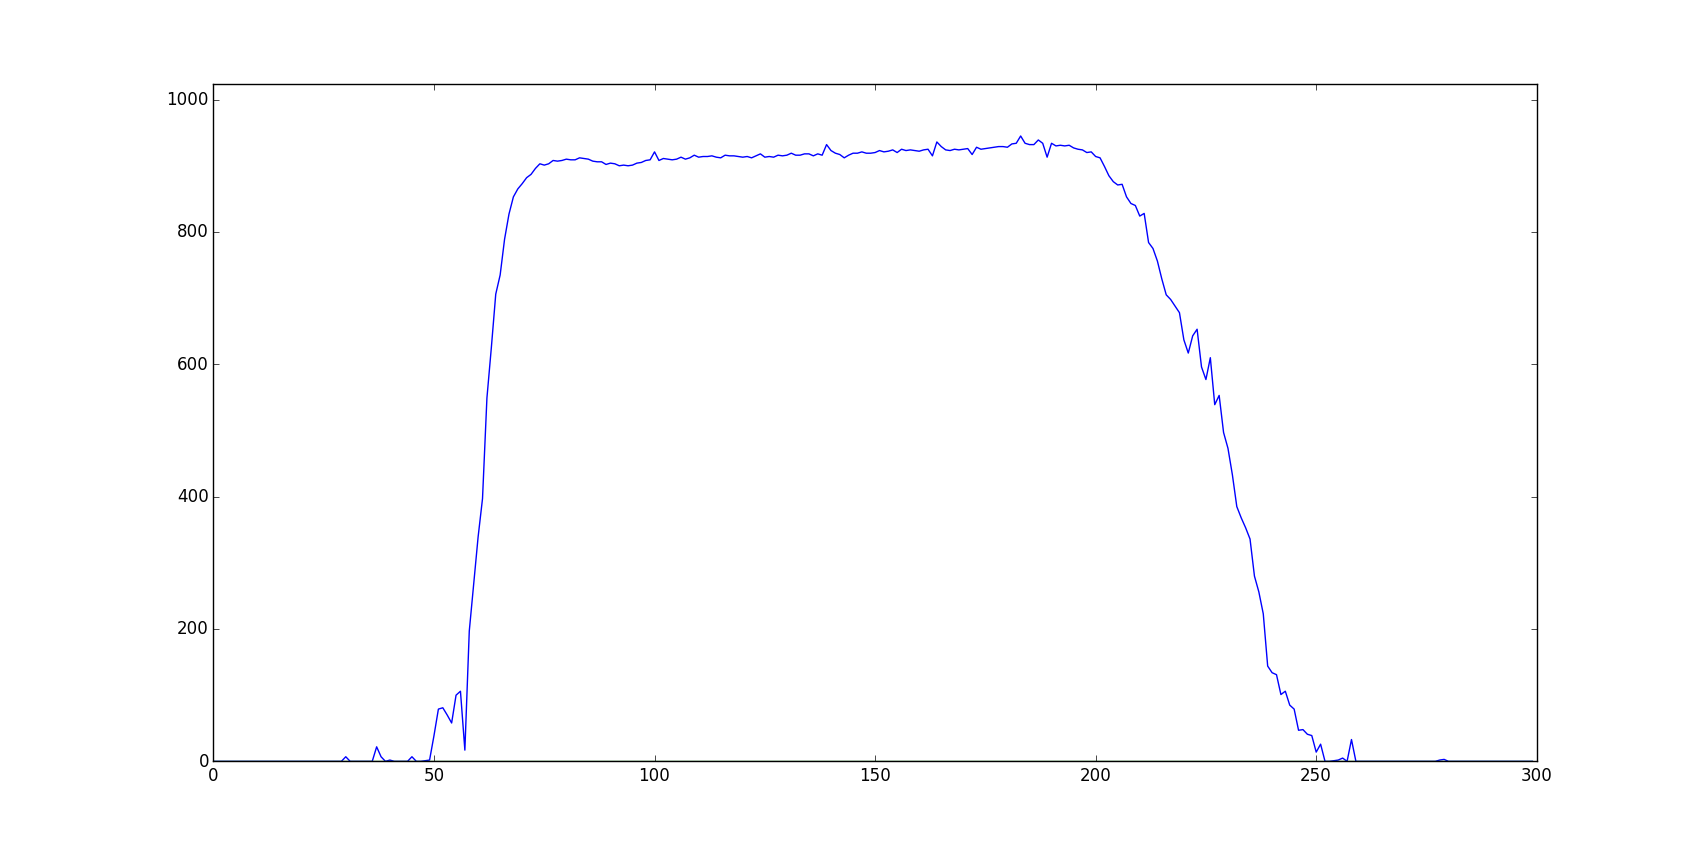
\includegraphics[width=0.75\textwidth]{FSR_Linearity}}
    \end{figure}

    From these readings it can be seen that there is a non-linear relationship
    between applied preassure and measurement. As the voltage measured is
    proportional to the inverse of the FSR resistance \parencite{ada2016},
    voltage increases at what appears to be an exponentially decreasing rate as
    resistance increase at the same rate.

    \section{Using the FSR values to create a tone}
    Building on the circuit developed in step 1, a speaker was attached. The
    speaker was connected to digital output 8 and to ground. Code was written
    to read input from the FSR, scale values to fall between pre-determined
    high and low values, and output a tone of the frequency specified for 20ms. 
    The result is an instrument that outputs rapid short tones that increase in
    pitch based on pressure applied.

    \begin{figure}[H]
        \makebox[\textwidth]{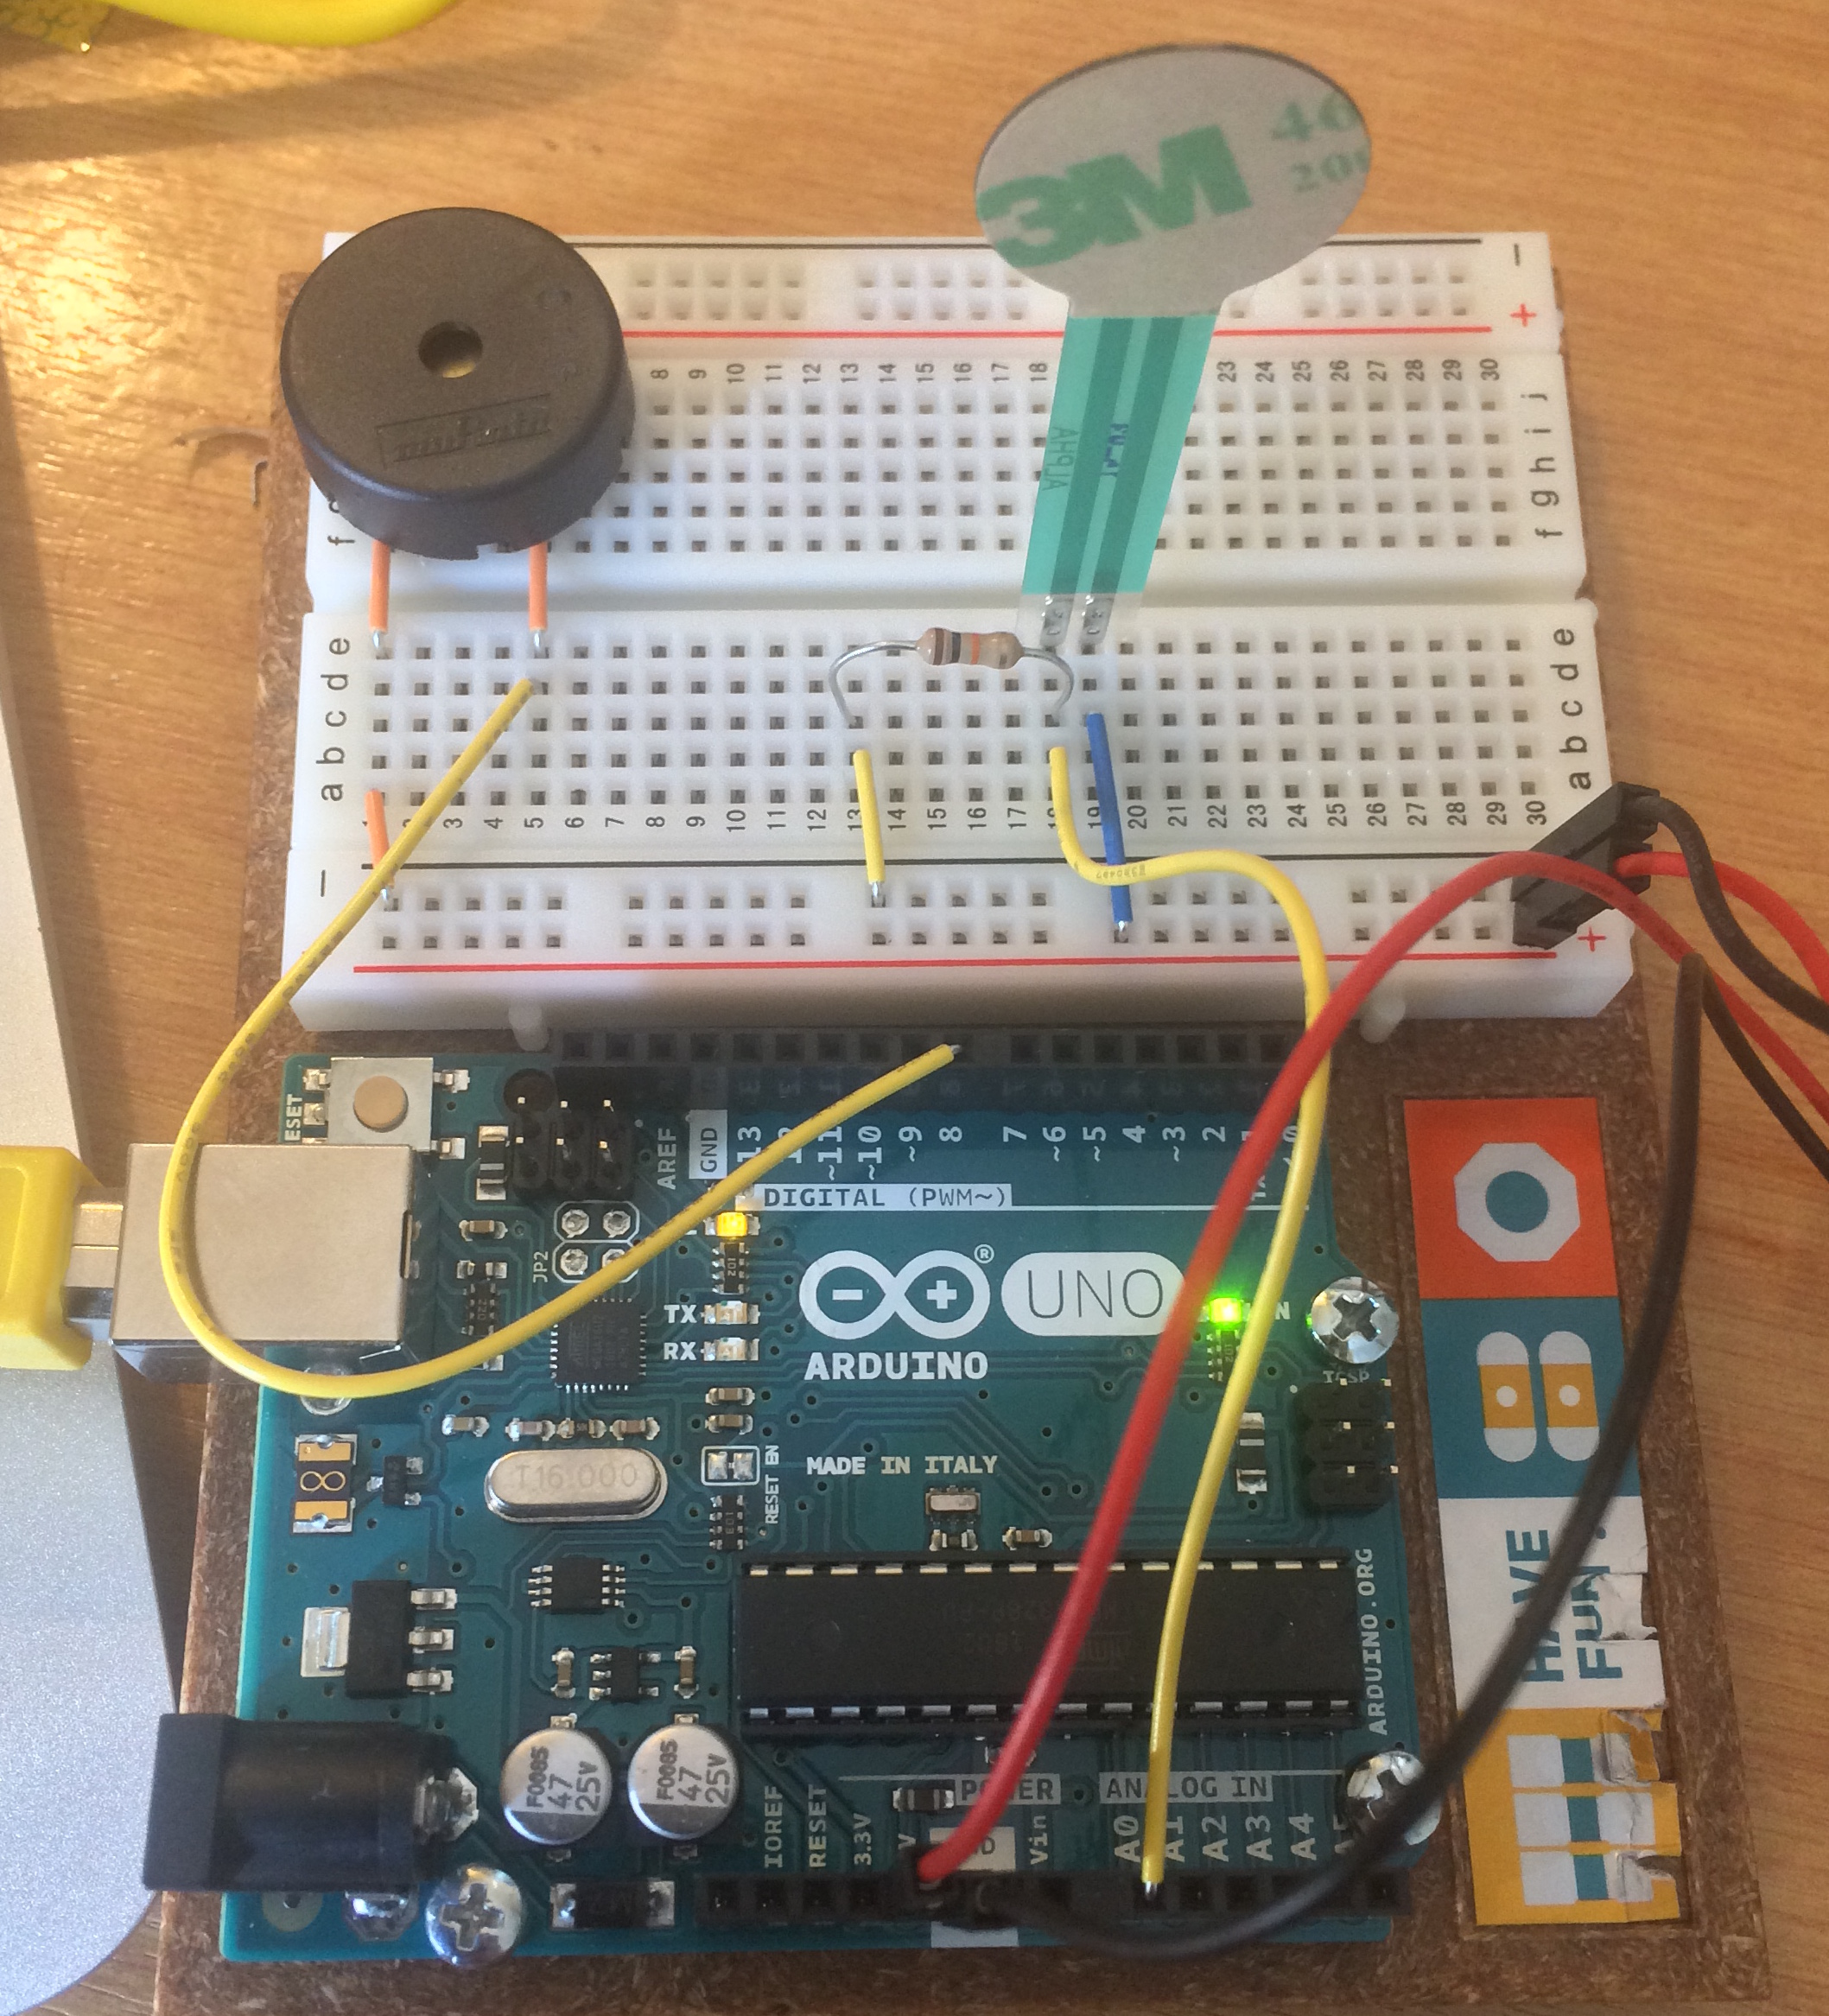
\includegraphics[width=0.35\textwidth]{Step2}}
    \end{figure}

    The speaker is capable of producing tones as low as around 100hz. Below
    this, the tone begins to lose it's tonal quality and the rhythmic
    characteristics become more prominent. The speaker can also produce tones
    as high as around 10Khz, however perceived loudness deteriorates beyond
    5-6Khz.\\
    The instruments is capable of producing interesting melodies and has a
    tactile response. However the lack of control over amplitude and the
    inacuracy of the resistor result in difficulties when trying to perform a
    sequence of specific notes. This could be improved reducing the range of
    playable frequencies. This would allow for greater pitch accuracy at a cost
    of a lower range of possible tones.

    \section{Using buttons to make a simple keyboard}
    Buttons were then added to the instrument. This allows a user to play 8
    tones in a chromatic scale. Each button was attached to the circuit in a
    similar fashion to that of the FSK. Pull down reseistors were used and each
    buton was assigned a digital input, allowing the arduino to determine the
    state of the button as being on (HIGH) or off (LOW). Although this method
    worked corectly, an alternative method using a "resistor ladder" is
    detailed in the arduino manual. This would allow for the same performance,
    whilst using only one analog input as opposed to the 8 digital inputs as
    used in this implementation.
    The arduino was then programmed to iterate across buttons until an active
    button was found. An array of note frequencies would then be accessed by
    index to determine the button's note frequency. This could then be played
    through the built in tone function using the speaker.\\

    \begin{figure}[H]
        \makebox[\textwidth]{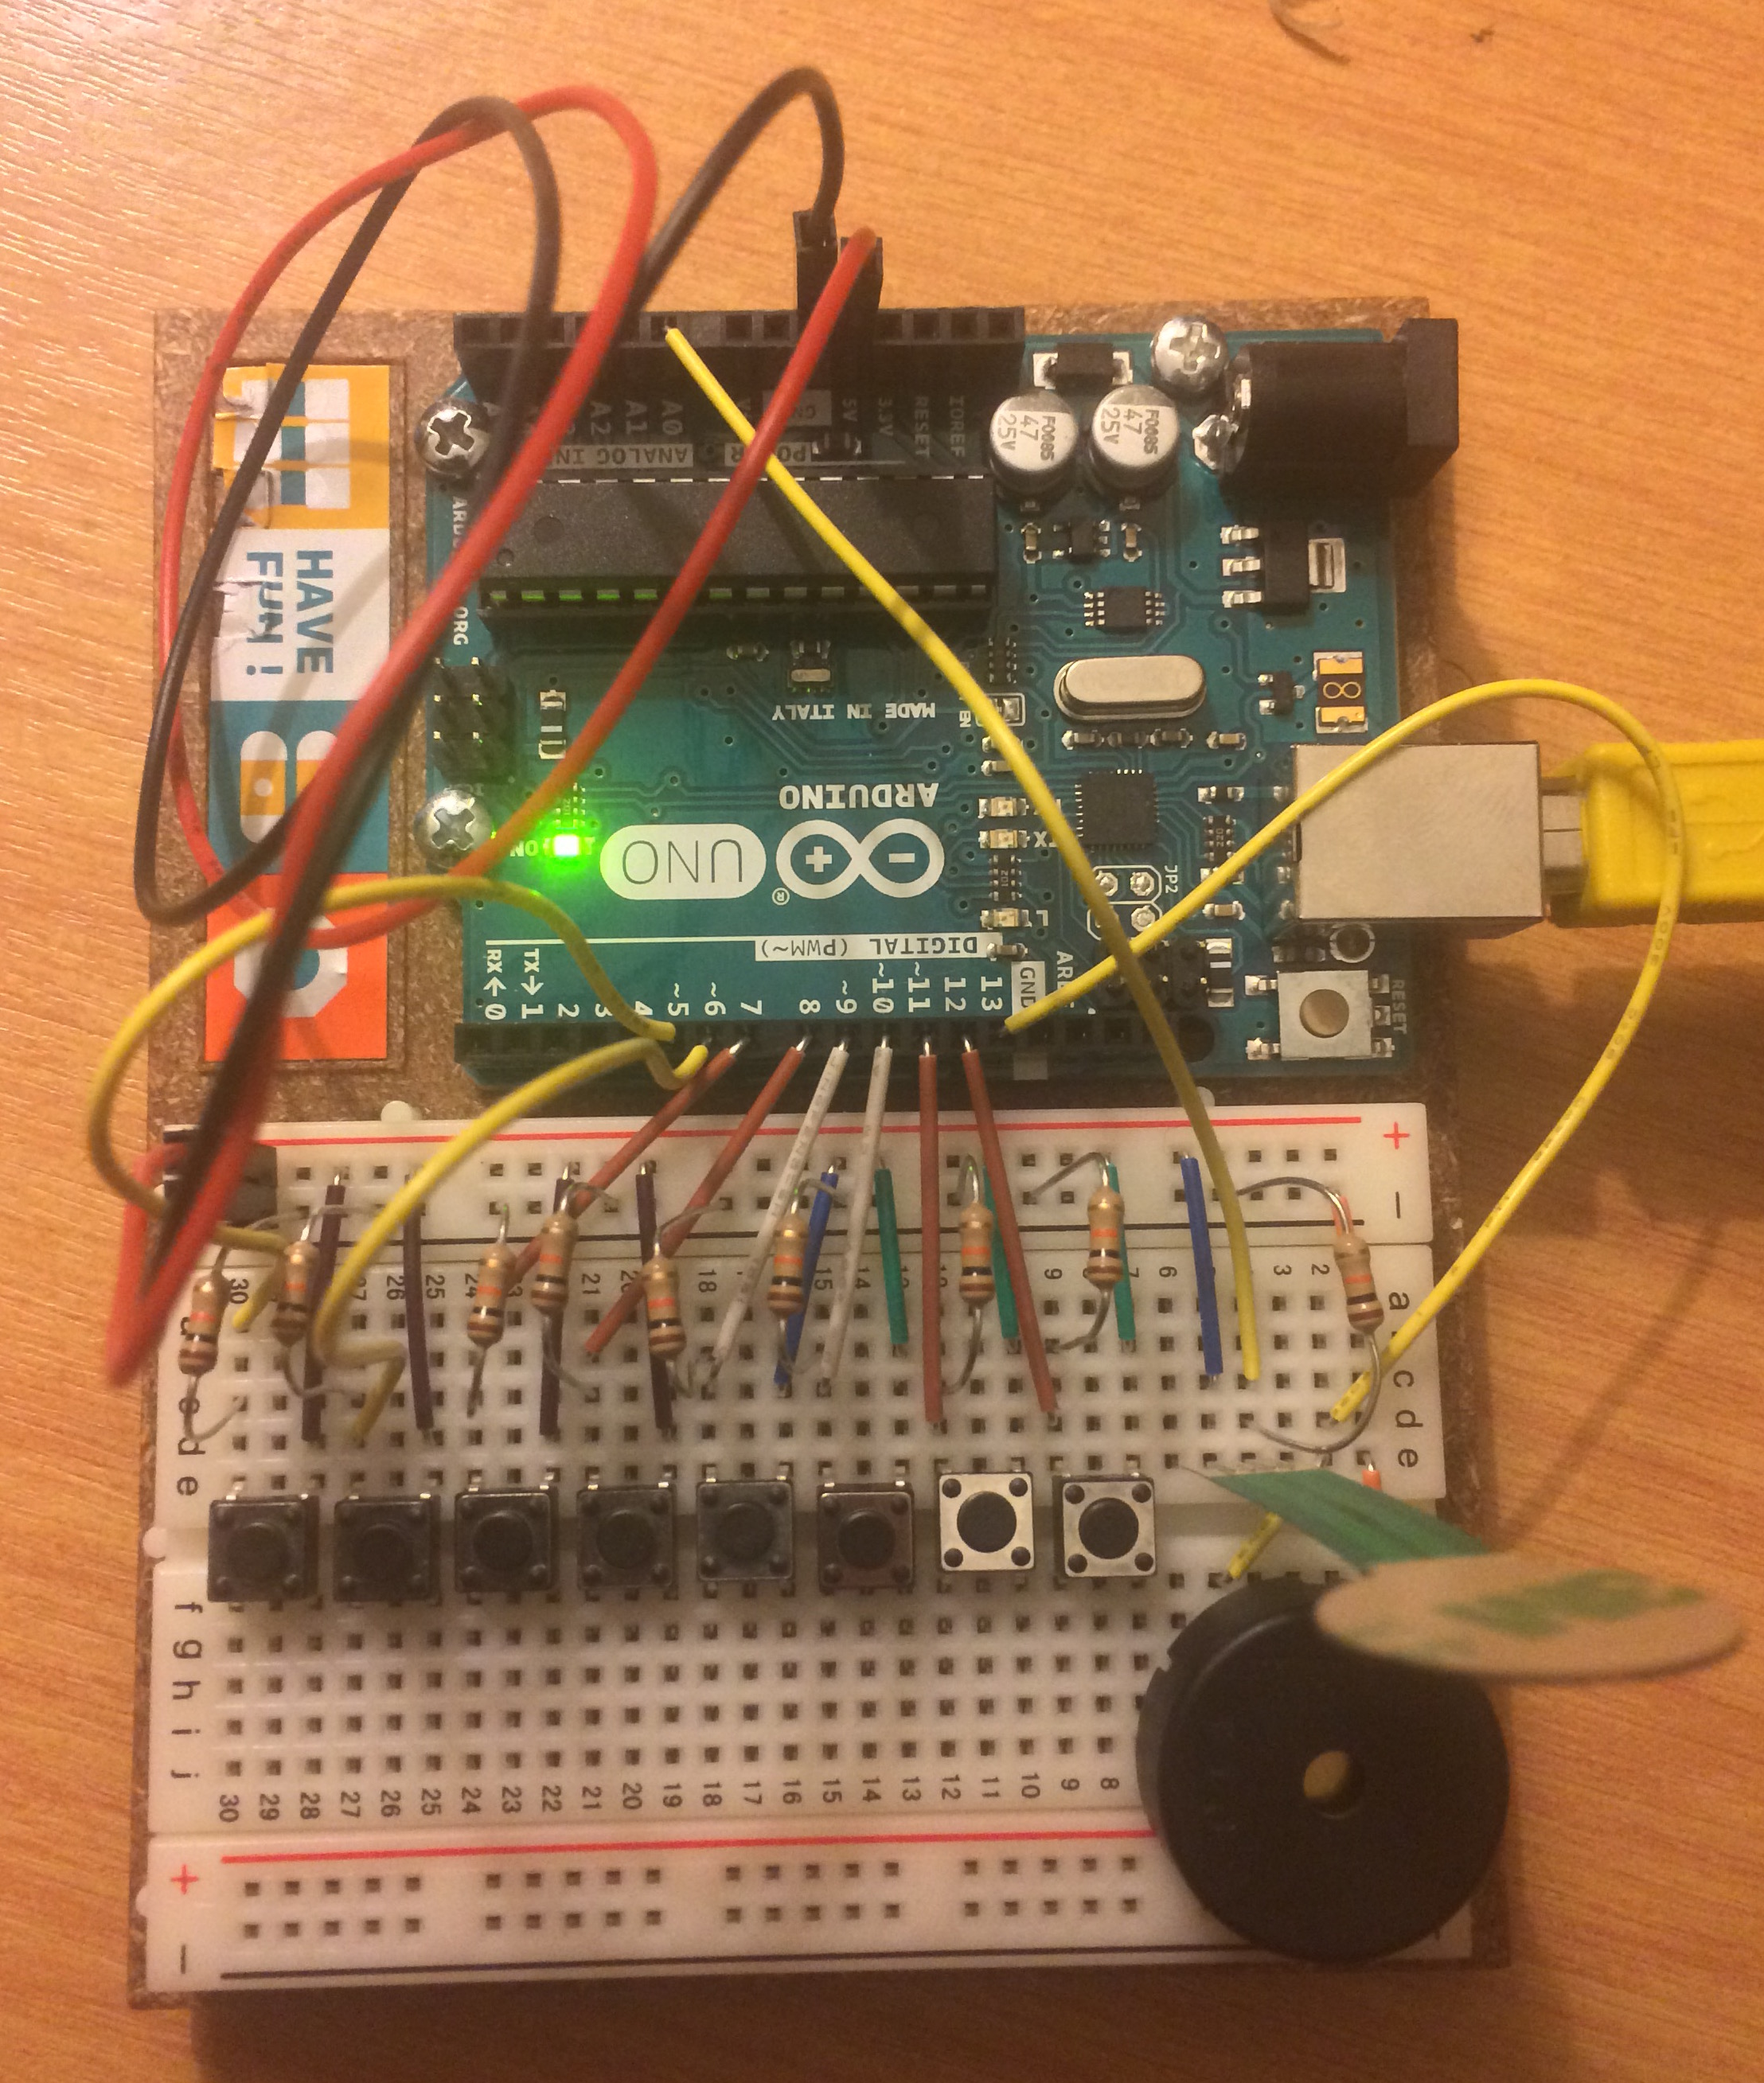
\includegraphics[width=0.35\textwidth]{Step3}}
    \end{figure}

    The instrument is now able to play precise tones with far greater accuracy
    than it was using the FSR. However, this comes at the cost of the tactile
    and expressive control offered by the FSR. The limit of available notes and
    lack of touch sensitivity make for an unintuitive playing experience.
    \section{Adding vibrato using the FSR}


    \printbibliography
\end{document}
